The simplicity of the instability criterion, Eq.~\eqref{eq:r_condition}, makes the necessary conditions for thermohaline mixing in stellar interiors readily identifiable. 
However, predicting the efficiency of thermohaline mixing is much more challenging. 
Due to the diffusive, small-scale nature of thermohaline mixing, a diffusive approximation is commonly taken for the turbulent mixing of chemicals and heat, so that the total mixing of chemical species, say, is given by the sum of the molecular diffusivity and some turbulent mixing coefficient $\Dth$ (the turbulent mixing of heat is often assumed to be negligible relative to radiative diffusion). \textcolor{red}{[Uhoh! Does the following sentence belong here or in the previous section??]}
This quantity can be converted to the compositional Nusselt number $\Numu$ discussed in the fluid dynamics literature using the formula
\begin{equation} \label{eq:Dth_from_Nu}
    \Dth = (\Numu - 1)\kappa_\mu.
\end{equation}

We refer to any model that predicts $\Dth$ as a function of stellar structure variables (e.g.~gradients and molecular diffusivities of chemicals and heat) as a (parameterized) mixing model or mixing prescription. 
Such mixing prescriptions have been implemented in a variety of stellar evolution codes \citep[see][and references therein]{lattanzio_etal_2015}, enabling studies of the effects of thermohaline mixing in stars across the HR diagram.

Efforts to develop thermohaline mixing prescriptions for use in modeling stellar interiors date back to the 1970's \citep{ulrich_1972}, and have ranged in sophistication from arguments based on dimensional analysis, to analytical derivations informed by hydrodynamic simulations \textcolor{red}{[too harsh?]}. 
The reader is again referred to \citet{garaud_DDC_review_2018} for a comprehensive review of efforts to predict mixing efficiency -- here, we briefly summarize the most commonly used and more recently developed prescriptions.

%Of the mixing models implemented in MESA, the earliest is due to \citet{ulrich_1972} and \citet{kippenhahn_etal_1980} \textcolor{red}{[check refs]}

The default \textcolor{red}{[no longer default apparently. earliest? most commonly used?]} thermohaline mixing model in the MESA software instrument \citep{mesa2} was originally derived by \citet{ulrich_1972, kippenhahn_etal_1980}.
%Thermohaline mixing is treated as a diffusion process, with a diffusion coefficient
Using arguments based on dimensional grounds and assumptions about the shape and motion of fluid ``blobs", they predicted a mixing efficiency of the form
\begin{equation} \label{eq:Dth-kipp}
    \Dth = C_t \kappa_T R_0^{-1},
\end{equation}
\citep[see Eq.~(5) of][]{charbonnel_thermohaline_2007}
where $C_t$ is a free parameter, with plausible values ranging from $C_t = 658$ \citep{ulrich_1972} to $C_t = 12$ \citep{kippenhahn_etal_1980}. 
\citet{charbonnel_thermohaline_2007} used a value of $C_t = 1000$ in stellar evolution models and found chemical mixing trends that were broadly consistent with observational data from \citet{Gratton2000}.

Equation \eqref{eq:Dth-kipp} is implemented in MESA as
\begin{equation} \label{eq:Dth-kipp-MESA}
    \Dth = \alpha_{\rm{th}} \frac{3 K}{2\rho C_P}R_0^{-1}
\end{equation}
\citep[see Eq.~(14) of][]{mesa2}. 
Here, $\alpha_{\rm{th}}$ is a dimensionless efficiency parameter related to $C_t$ by $C_t = 3\alpha_{\rm{th}}/2$, $K$ is the radiative conductivity, $\rho$ is the density, and $C_P$ is the specific heat at constant pressure, with $\kappa_T = K/(\rho C_P)$. 
\textcolor{red}{[Point to green line in Fig.~\ref{fig:parameterization_compare} now, or later after all the parameterizations have been introduced?]}

While 1D stellar evolution models from \citet{charbonnel_thermohaline_2007} using Eq.~\eqref{eq:Dth-kipp} with $C_t = 1000$ reproduced trends that are consistent with observational data from \citet{Gratton2000}, this value is orders of magnitude larger than the efficiency of thermohaline mixing suggested by \citet{kippenhahn_etal_1980}. 
Furthermore, Eq.~\eqref{eq:Dth-kipp} predicts finite mixing for $R_0 \geq 1/\tau$ ($r \geq 1$), even though the instability driving thermohaline mixing is stabilized for these parameters. 
As reviewed by \citet{garaud_DDC_review_2018}, these concerns motivated the use of multidimensional simulations by multiple groups as a form of numerical experiment to more precisely estimate mixing efficiency \citep{Denissenkov2010thermohaline,traxler_etal_2011}. 
%\citet{traxler_etal_2011} and \citet{brown_etal_2013} performed 3D hydrodynamic simulations across a broad range of parameters and broadly found that the mixing efficiency parameter required in \citet{charbonnel_thermohaline_2007} to find agreement with observations was orders of magnitude larger than what is found in simulations, suggesting thermohaline mixing may be unable to explain observations of extra mixing.
\citet{traxler_etal_2011} and \citet{brown_etal_2013} performed 3D hydrodynamic simulations across a broad range of parameters and developed mixing prescriptions that fit their simulations. 
%They found that mixing efficiency is most easily discussed in terms of $r$.
\citet{traxler_etal_2011} derived a mixing law by fitting an analytic function to their simulations.
%They define the reduce density ratio, $r \equiv (R_0 - 1)/(\tau^{-1} - 1)$, where $\tau = \kappa_\mu/\kappa_T$ is the ratio of compositional to thermal diffusivity.
They find that
\begin{equation} \label{eqn:trax_model}
   \Dth = \kappa_{\mu}\sqrt{\frac{\mathrm{Pr}}{\tau}}\left(a e^{-br}[1 - r]^c\right),
\end{equation}
where $\mathrm{Pr} = \nu / \kappa_T$ is the Prandtl number, with $\nu$ the viscosity, and they find $a = 101 \pm 1$, $b = 3.6 \pm 0.3$, and $c = 1.1 \pm 0.1$ by fitting to simulation results. \textcolor{red}{[Now that we've removed it from the rest of the paper, should we drop the actual formula for the Traxler model? Or should we include it since it's still in MESA?]}

\citet{brown_etal_2013} note that the model in Eqn.~\eqref{eqn:trax_model} performs well at high $R_0$, but underestimates mixing at low $R_0$, particularly in the stellar regime of low Pr and $\tau$.
They develop a semi-analytical model for thermohaline mixing,
\begin{equation}
    \Dth = \kappa_{\mu}C^2\frac{\lambda^2}{\tau l^2(\lambda + \tau l^2)},
    \label{eqn:brown_model}
\end{equation}
where $\lambda$ is the growth rate of the fastest-growing linearly unstable mode, $l$ is its horizontal wavenumber, and $C \approx 7$ was fit to simulation data.
The values of $\lambda$ and $l$ are obtained by finding the roots of a cubic and quadratic polynomial (their Eqs.~19 and 20).
The prescription Eq.~\eqref{eqn:brown_model} has since been used in \citep{bauer_bildsten_2019} and other works \textcolor{red}{[do we put the MESA version where this was first implemented?]}.

\textcolor{red}{[BRING IT BACK TO THE ISSUE OF $C_t$ AND LARGE VS SMALL VALUES BEFORE MOVING ON TO MHD]}

%\citet{harrington} build on the model of \citet{brown_etal_2013} by including the effects of initially uniform, vertical magnetic fields. 
\citet{harrington} extended the work of \citet{brown_etal_2013} by performing 3D magnetohydrodynamic (MHD) simulations of thermohaline mixing at $r = 0.05$ with initially uniform, vertical magnetic fields of various strengths to approximate the effects of magnetic fields from external processes, e.g., a global dipole field or a large-scale magnetic field left by a dynamo process from the receding convective envelope \textcolor{red}{[TMI]}. 
They found that magnetism increases mixing efficiency, sometimes dramatically.
They developed a mixing prescription that accounts for this effect by building on the model of \citet{brown_etal_2013}, Eq.~\eqref{eqn:brown_model}.
The strength of the magnetic field is introduced into their model through their parameter $H_B$, which is proportional to the square of the magnetic field strength and depends on other stellar structure variables \citep[see
\begin{equation} \label{eq:HB}
    H_B =
\end{equation}
Their mixing prescription is of the form
\begin{equation} \label{eq:harrington_model}
    \Dth = \kappa_{\mu}K_B\frac{w_f^2}{\tau (\lambda + \tau l^2)},
\end{equation}
where $w_f$ is obtained by solving a quartic polynomial that includes the magnetic field strength. 
This model reduces to Eq
%Their Eqn.~32 provides an expression for $\hat{w}_f^2$ which depends on the magnitude of the magnitude field $B_0^2$.
This expression has two asymptotic limits, in which $\hat{w}_f^2 \propto B_0^2$ when $B_0$ is large, and which reduces exactly to the model of \citet{brown_etal_2013} when $B_0$ is small.
(this is a new model that is not yet implemented in MESA).


There has been other work regarding multi-D models of thermohaline mixing \citep{denissenkov_2010, denissenkov_merryfield_2011}, but 2D thermohaline behaves very differently from 3D thermohaline \citep{garaud_brummell_2015}, and so we do not consider that set of data in this work.

\citet{lattanzio_etal_2015} tested one or multiple of these models in a bunch of different codes on the RGB and found X.
In this paper, we will determine if observations are capable of probing the differences between these different models are not.

\begin{figure}
    \centering
    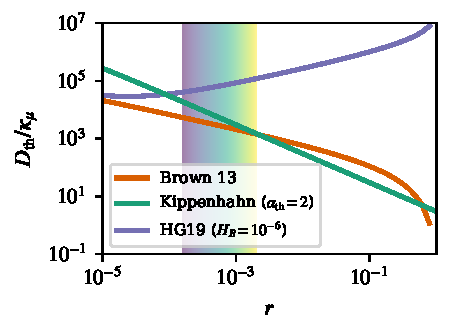
\includegraphics[width=\columnwidth]{Nu_models_comparison.pdf}
    \caption{\textcolor{red}{[Todo: Write caption.]}}
    \label{fig:parameterization_compare}
\end{figure}
